% \hiddenchapter{분석 산출물}
% \ChapterTitle[\thechapter]{분석 산출물}
%%% See Preamble for an explanation of both of these %%%

\setcounter {section}{0}

% \hiddensection{업무 분석: Use Case Modeling}
% \SectionTitle{\thesection}{업무 분석 : Use Case Modeling}

\begin{landscape}
    \hiddenchapter{분석 산출물}
    \ChapterTitle[\thechapter]{분석 산출물}

    \hiddensection{업무 분석: Use Case Modeling}
    \SectionTitle{\thesection}{업무 분석 : Use Case Modeling}

    % \begin{itemize}
    %     \item[] \textbf{현업 요구사항 정의서}
    % \end{itemize}

    \small
    \arrayrulecolor{black}
    \begin{longtable}
        {
            |>{\centering\hspace{0pt}}m{0.035\linewidth}
            |>{\centering\hspace{0pt}}m{0.050\linewidth}
            |>{\centering\hspace{0pt}}m{0.045\linewidth}
            |>{\centering\hspace{0pt}}m{0.050\linewidth}
            |>{\centering\hspace{0pt}}m{0.070\linewidth}
            |>{\hspace{0pt}}m{0.255\linewidth}
            |>{\centering\hspace{0pt}}m{0.135\linewidth}
            |>{\centering\hspace{0pt}}m{0.090\linewidth}
            |>{\centering\hspace{0pt}}m{0.050\linewidth}
            |>{\hspace{0pt}}m{0.040\linewidth}|
        } 
        \hline
        \multicolumn{10}{|c|}{\cellcolor{aliceblue}{}} \\
        \multicolumn{10}{|c|}{\cellcolor{aliceblue}{\Large\textbf{현 업 요 구 사 항 정 의 서}}} \\
        \multicolumn{10}{|c|}{\cellcolor{aliceblue}{}} \\
        \hline
        \rowcolor{aliceblue} 
        \multicolumn{5}{|c}{\cellcolor{aliceblue}{\normalsize{시스템 명: Travel Diary}}}
        & \multicolumn{1}{c}{}
        & \multicolumn{2}{c}{\cellcolor{aliceblue}{\normalsize{작성일: 2020년 12월 21일}}}
        & \multicolumn{2}{c|}{\normalsize{작성자: 왕밤빵}} \\ \hline
        \rowcolor{aliceblue} 서브 시스템 
        & 요구사항 ID & 유형 & 업무명 & 세부 기능 
        & \multicolumn{1}{>{\centering\hspace{0pt}}m{0.255\linewidth}|}{처리내용} 
        & 입력자료 & 출력자료 & 수용여부 
        & \multicolumn{1}{>{\centering\arraybackslash\hspace{0pt}}m{0.040\linewidth}|}{비고} \\* \hline
        \endfirsthead \hline
        \rowcolor{aliceblue} 서브 시스템 & 요구사항 ID & 유형 & 업무명 & 세부 기능 & \multicolumn{1}{>{\centering\hspace{0pt}}m{0.255\linewidth}|}{처리내용} & 입력자료 & 출력자료 & 수용여부 & \multicolumn{1}{>{\centering\arraybackslash\hspace{0pt}}m{0.040\linewidth}|}{비고} \\* \hline 
        \endhead
        {\cellcolor{aliceblue}} & \multicolumn{9}{>{\hspace{0pt}}m{0.885\linewidth}|}{ USER } \\* \hhline{|>{\arrayrulecolor{aliceblue}}->{\arrayrulecolor{black}}|-|-|-|-|-|-|-|-|-|}
        {\cellcolor{aliceblue}} & R101 & 기능 & \multirow{5}[30]{=}{\Centering{}자사 회원가입} & 정보 입력 & 필수 입력조건으로 e-mail, 비밀번호, 닉네임, 이름, 핸드폰번호. 선택 입력조건으로 거주지(시, 구), 관심 여행지역(나라, 도시), 생년월일, 프로필 사진을 기입한다. & e-mail, 비밀번호, 닉네임, 이름, 핸드폰 번호, 거주지, 관심 여행지역, 생년월일, 프로필사진, 가입날짜 & 닉네임, 환영 메세지 & o & \multicolumn{1}{>{\Centering\hspace{0pt}}m{0.040\linewidth}|}{} \\* \hhline{|>{\arrayrulecolor{aliceblue}}->{\arrayrulecolor{black}}|-|-|~|-|-|-|-|-|-|}
        {\cellcolor{aliceblue}} & \multirow{2}[4]{=}{\Centering{}R102} & \multirow{2}[4]{=}{\Centering{}기능} &  & \multirow{2}[4]{=}{\Centering{}중복체크} & 동일한 e-mail로 2개의 계정을 가입하지 못하도록 e-mail 중복체크를 하고 e-mail은 회원 아이디로 사용된다. & e-mail & 중복 여부 메세지 & o & \multicolumn{1}{>{\Centering\hspace{0pt}}m{0.038\linewidth}|}{} \\* \hhline{|>{\arrayrulecolor{aliceblue}}->{\arrayrulecolor{black}}|~|~|~|~|-|-|-|-|-|}
        {\cellcolor{aliceblue}} &  &  &  &  & 동일한 닉네임 설정이 불가능 하도록 닉네임의 중복 체크를 한다. & 닉네임 & 중복 여부 메세지 & o & \multicolumn{1}{>{\Centering\hspace{0pt}}m{0.038\linewidth}|}{Ajax} \\* \hhline{|>{\arrayrulecolor{aliceblue}}->{\arrayrulecolor{black}}|-|-|~|-|-|-|-|-|-|}
        \multirow{-3}{=}{{\cellcolor{aliceblue}}\Centering{}회원관리} & R103 & 기능 &  & SMS 문자 인증 & 핸드폰 번호 1개 당 하나의 아이디만 생성할 수 있도록 체크를 하고 본인 확인을 위한 sms 인증을 진행한다. & 전화번호, 인증번호 & 중복 여부 메세지, 본인확인 메세지 & o & \multicolumn{1}{>{\Centering\hspace{0pt}}m{0.038\linewidth}|}{청기와 Lab} \\* \hhline{|>{\arrayrulecolor{aliceblue}}->{\arrayrulecolor{black}}|-|-|~|-|-|-|-|-|-|}
        {\cellcolor{aliceblue}} & R104 & 기능 &  & 이메일 인증 & 본인의 e-mail이 맞는지 확인을 위한 인증을 진행한다. & e-mail, 인증번호 & 본인확인 메세지 & o & \multicolumn{1}{>{\Centering\hspace{0pt}}m{0.038\linewidth}|}{} \\* \hhline{|>{\arrayrulecolor{aliceblue}}->{\arrayrulecolor{black}}|-|-|-|-|-|-|-|-|-|}
        {\cellcolor{aliceblue}} &  &  &  & Google & Google 계정으로 회원가입 가능. 계정 로그인 시 계정 연동 동의 체크 화면이 노출되며 '동의' 시 정보 입력으로 이동 & Google 아이디, 비밀번호, 닉네임, 이름, 핸드폰 번호, 거주지, 관심 여행지역, 생년월일, 프로필사진, 가입날짜 & 닉네임, 환영 메세지 & o & \multicolumn{1}{>{\Centering\hspace{0pt}}m{0.038\linewidth}|}{Google Login Api} \\* \hhline{|>{\arrayrulecolor{aliceblue}}->{\arrayrulecolor{black}}|~|~|~|-|-|-|-|-|-|}
        {\cellcolor{aliceblue}} & \multirow{2}{=}{\Centering{}R105} & \multirow{2}{=}{\Centering{}기능} & \multirow{2}{=}{\Centering{}소셜 연동 회원가입} & Kakao & Kakao 계정으로 회원가입 가능. 계정 로그인 시 계정 연동 동의 체크 화면이 노출되며 '동의' 시 정보 입력으로 이동 & Kakao 아이디, 비밀번호, 닉네임, 이름, 핸드폰 번호, 거주지, 관심 여행지역, 생년월일, 프로필사진, 가입날짜 & 닉네임, 환영 메세지 & o & \multicolumn{1}{>{\Centering\hspace{0pt}}m{0.038\linewidth}|}{Kakao Login Api} \\* \hhline{|>{\arrayrulecolor{aliceblue}}->{\arrayrulecolor{black}}|~|~|~|-|-|-|-|-|-|}
        {\cellcolor{aliceblue}} &  &  &  & Naver & Naver 계정으로 회원가입 가능. 계정 로그인 시 계정 연동 동의 체크 화면이 노출되며 '동의' 시 정보 입력으로 이동 & Naver 아이디, 비밀번호, 닉네임, 이름, 핸드폰 번호, 거주지, 관심 여행지역, 생년월일, 프로필사진, 가입날짜 & 닉네임, 환영 메세지 & o & \multicolumn{1}{>{\Centering\hspace{0pt}}m{0.038\linewidth}|}{Naver Login Api} \\* \hhline{|>{\arrayrulecolor{aliceblue}}->{\arrayrulecolor{black}}|-|-|-|-|-|-|-|-|-|}
        {\cellcolor{aliceblue}} & \multirow{11}{=}{\Centering{}R106} & \multirow{11}{=}{\Centering{}기능} & \multirow{19}{=}{\Centering{}로그인} & 계정 로그인 & 자사 사이트에서 가입한 계정으로 로그인 & e-mail, 비밀번호 &  & o & \multicolumn{1}{>{\Centering\hspace{0pt}}m{0.038\linewidth}|}{} \\* \hhline{|>{\arrayrulecolor{aliceblue}}->{\arrayrulecolor{black}}|~|~|~|-|-|-|-|-|-|}
        {\cellcolor{aliceblue}} &  &  &  & Google & Google 계정으로 로그인 & Google 아이디, 비밀번호 &  & o & \multicolumn{1}{>{\Centering\hspace{0pt}}m{0.038\linewidth}|}{Google Login Api} \\* \hhline{|>{\arrayrulecolor{aliceblue}}->{\arrayrulecolor{black}}|~|~|~|-|-|-|-|-|-|}
        {\cellcolor{aliceblue}} &  &  &  & Kakao & Kakao 계정으로 로그인 & Kakao 아이디, 비밀번호 &  & o & \multicolumn{1}{>{\Centering\hspace{0pt}}m{0.038\linewidth}|}{Kakao Login Api} \\* \hhline{|>{\arrayrulecolor{aliceblue}}->{\arrayrulecolor{black}}|~|~|~|-|-|-|-|-|-|}
        {\cellcolor{aliceblue}} &  &  &  & Naver & Naver 계정으로 로그인 & Naver 아이디, 비밀번호 &  & o & \multicolumn{1}{>{\Centering\hspace{0pt}}m{0.038\linewidth}|}{Naver Login Api} \\* \hhline{|>{\arrayrulecolor{aliceblue}}->{\arrayrulecolor{black}}|-|-|~|-|-|-|-|-|-|}
        \multirow{-2}{=}{{\cellcolor{aliceblue}}\Centering{}회원관리} & R107 & 기능 &  & 아이디 저장 & 체크박스 선택 시 사이트 방문하여 로그인 할 때 아이디가 저장된다. &  &  & o & \multicolumn{1}{>{\Centering\hspace{0pt}}m{0.038\linewidth}|}{} \\* \hhline{|>{\arrayrulecolor{aliceblue}}->{\arrayrulecolor{black}}|-|-|~|-|-|-|-|-|-|}
        {\cellcolor{aliceblue}} & R108 & 기능 &  & 로그인 상태 유지 & 체크박스 선택 시 사이트 방문할 때 로그인 상태가 유지된다. &  &  & o & \multicolumn{1}{>{\Centering\hspace{0pt}}m{0.038\linewidth}|}{} \\* \hhline{|>{\arrayrulecolor{aliceblue}}->{\arrayrulecolor{black}}|-|-|~|-|-|-|-|-|-|}
        {\cellcolor{aliceblue}} & R109 & 기능 &  & 아이디(e-mail) 찾기 & sms 인증을 통해 본인 확인이 완료되면 아이디를 보여준다. & 전화번호, 인증번호, 이름 & 아이디(e-mail) & o & \multicolumn{1}{>{\Centering\hspace{0pt}}m{0.038\linewidth}|}{} \\* \hhline{|>{\arrayrulecolor{aliceblue}}->{\arrayrulecolor{black}}|-|-|~|-|-|-|-|-|-|}
        {\cellcolor{aliceblue}} & R110 & 기능 &  & 비밀번호 찾기 & sms 인증을 통해 본인 확인이 완료되면 비밀번호 재설정 페이지로 넘어간다. & 아이디(e-mail), 전화번호, 인증번호 &  & o & \multicolumn{1}{>{\Centering\hspace{0pt}}m{0.038\linewidth}|}{} \\* \hhline{|>{\arrayrulecolor{aliceblue}}->{\arrayrulecolor{black}}|-|-|-|-|-|-|-|-|-|}
        {\cellcolor{aliceblue}} & R111 & 기능 & 로그아웃 & 로그아웃 & 로그아웃이 이루어진다. &  & 로그아웃 메세지 & o & \multicolumn{1}{>{\Centering\hspace{0pt}}m{0.038\linewidth}|}{} \\* \hhline{|>{\arrayrulecolor{aliceblue}}->{\arrayrulecolor{black}}|-|-|-|-|-|-|-|-|-|}
        {\cellcolor{aliceblue}} & R112 & 기능 & \multirow{6}{=}{\Centering{}내 정보 관리} & 내 정보 조회 & 로그인한 사용자는 내 정보 조회를 통해 등록해 놓은 정보를 조회할 수 있다. & e-mail & e-mail, 비밀번호, 닉네임, 이름, 핸드폰 번호, 거주지, 관심 여행지역, 생년월일, 프로필사진 & o & \multicolumn{1}{>{\Centering\hspace{0pt}}m{0.038\linewidth}|}{} \\* \hhline{|>{\arrayrulecolor{aliceblue}}->{\arrayrulecolor{black}}|-|-|~|-|-|-|-|-|-|}
        {\cellcolor{aliceblue}} & R113 & 기능 &  & 내 정보 수정 & 개인 정보 수정 시 필수 정보는 비밀번호를 재입력하여 본인인증을 마친 후 각각의 항목들을 수정할 수 있고 선택 정보는 본인인증 없이 수정 가능하다. 각각의 항목들은 팝업창을 통해 하나하나 수정, 저장할 수 있다. & e-mail, 비밀번호, 닉네임, 이름, 핸드폰 번호, 거주지, 관심 여행지역, 생년월일 & 수정 완료 메세지 & o & \multicolumn{1}{>{\Centering\hspace{0pt}}m{0.038\linewidth}|}{} \\* \hhline{|>{\arrayrulecolor{aliceblue}}->{\arrayrulecolor{black}}|-|-|~|-|-|-|-|-|-|}
        {\cellcolor{aliceblue}} & R114 & 기능 &  & 회원 탈퇴 & 회원 탈퇴는 본인인증(sms 인증)을 마친 후에 비활성화할 수 있고 비활성화가 1달동안 지속되면 영구 삭제가 된다. 1달 이내에 재접속 시에 계정은 복구된다. & 핸드폰 번호, 인증번호, e-mail, 계정 활성화 여부코드 & 회원탈퇴 재확인 메세지, 탈퇴 완료 메세지 & o & \multicolumn{1}{>{\Centering\hspace{0pt}}m{0.038\linewidth}|}{플래그 처리} \\* \hhline{|>{\arrayrulecolor{aliceblue}}->{\arrayrulecolor{black}}|---------|}
        {\cellcolor{aliceblue}} & \multicolumn{9}{>{\hspace{0pt}}m{0.885\linewidth}|}{ ADMIN } \\* \hhline{|>{\arrayrulecolor{aliceblue}}->{\arrayrulecolor{black}}|-|-|-|-|-|-|-|-|-|}
        \multirow{-10}{=}{{\cellcolor{aliceblue}}\Centering{}회원관리} & R115 & 기능 & \multirow{4}{=}{\Centering{}관리자 권한} & 회원 정보 조회 & 관리자 계정으로 로그인 시 모든 회원의 정보를 조회할 수 있다. & e-mail & e-mail, 비밀번호, 닉네임, 이름, 핸드폰 번호, 거주지, 관심 여행지역, 생년월일, 프로필사진 & o & \multicolumn{1}{>{\Centering\hspace{0pt}}m{0.038\linewidth}|}{Ajax} \\* \hhline{|>{\arrayrulecolor{aliceblue}}->{\arrayrulecolor{black}}|-|-|~|-|-|-|-|-|-|}
        {\cellcolor{aliceblue}} & R116 & 기능 &  & 블랙리스트 회원 계정 정지 & 누적 신고 10회 이상이면 계정이 2주간 정지된다. & 신고 횟수, e-mail &  & o & \multicolumn{1}{>{\Centering\hspace{0pt}}m{0.038\linewidth}|}{} \\* \hline
        {\cellcolor{aliceblue}} & \multicolumn{9}{>{\hspace{0pt}}m{0.885\linewidth}|}{ USER } \\* \hhline{|>{\arrayrulecolor{aliceblue}}->{\arrayrulecolor{black}}|-|-|-|-|-|-|-|-|-|}
        {\cellcolor{aliceblue}} & R201 & 기능 &  & 지도에 등록 & 화면에 표시된 세계지도에 자신이 여행한 장소(범위 제한없이)를 선택하거나 검색하면 깃발로 표시되고 글을 등록할 수 있는 페이지로 넘어가게 된다. & 여행지 위치(GPS) &  & o & \multicolumn{1}{>{\Centering\hspace{0pt}}m{0.038\linewidth}|}{Google Map Api} \\* \hhline{|>{\arrayrulecolor{aliceblue}}->{\arrayrulecolor{black}}|-|-|~|-|-|-|-|-|-|}
        \multirow{2}{=}{{\cellcolor{aliceblue}}\Centering{}기록 관리} & R202 & 기능 &  &  & 작성자는 블로그 형식(자유롭게 글, 사진, 동영상을 올릴 수 있는 형식)으로 기록을 작성할 수 있다. & e-mail, 제목, 내용, 사진, 동영상, 등록 날짜, 기록 식별번호 & 등록 완료 메세지 & o &  \\* \hhline{|>{\arrayrulecolor{aliceblue}}->{\arrayrulecolor{black}}|-|-|~|~|-|-|-|-|-|}
        {\cellcolor{aliceblue}} & R203 & 기능 &  & \multirow{3}{=}{\Centering{}내용등록} & 작성자는 여행에서 사용한 지출 내역을 간단하게 작성할 수 있다. & 지출내역(지출 카테고리(교통비, 숙박비, 식비, 기타), 통화(원, 달러, 엔, 유로, 위안, 기타), 금액, 합계) &  & o & \multicolumn{1}{>{\Centering\hspace{0pt}}m{0.038\linewidth}|}{} \\* \hhline{|>{\arrayrulecolor{aliceblue}}->{\arrayrulecolor{black}}|-|-|~|~|-|-|-|-|-|}
        {\cellcolor{aliceblue}} & R204 & 기능 &  &  & 작성자는 여행 중 구매한 기념품의 사진과 간략한 설명을 등록할 수 있다. & 사진, 사진설명 글 &  & o & \multicolumn{1}{>{\Centering\hspace{0pt}}m{0.038\linewidth}|}{} \\* \hhline{|>{\arrayrulecolor{aliceblue}}->{\arrayrulecolor{black}}|-|-|~|~|-|-|-|-|-|}
        {\cellcolor{aliceblue}} & R205 & 기능 & \multirow{-5}{=}{\Centering{}기록 작성} &  & 작성자는 글에 어울리는 해시태그를 자유롭게 등록할 수 있다. 해시태그의 형식은 \#\textasciitilde{}\textasciitilde{}\textasciitilde{} {[}, \#\textasciitilde{}\textasciitilde{}\textasciitilde{}] 으로 작성할 수 있다. & \#\textasciitilde{}\textasciitilde{}\textasciitilde{} 형식의 해시태그 &  & o &  \\* \hhline{|>{\arrayrulecolor{aliceblue}}->{\arrayrulecolor{black}}|-|-|~|-|-|-|-|-|-|}
        {\cellcolor{aliceblue}} & R206 & 기능 &  & 후기 작성 & 내용 등록과 다르게 형식에 맞춰서 작성을 하며 여행지, 식당, 숙소 등의 간단한 한줄평과 평점을 남길 수 있다. & e-mail, 후기, 평점, 후기 식별번호 & 등록 완료 메세지 & o &  \\* \hhline{|>{\arrayrulecolor{aliceblue}}->{\arrayrulecolor{black}}|-|-|~|-|-|-|-|-|-|}
        {\cellcolor{aliceblue}} & R207 & 기능 &  & 공개 / 비공개 설정 & 작성지는 글을 등록할 때 공개 / 비공개 여부를 결정할 수 있다. 공개 선택 시 커뮤니티에서 다른 사람들이 볼 수 있고, 비공개 설정 시 자신 외에는 볼 수 없는 상태가 된다. & 공개 여부 식별번호 &  & o &  \\* \hhline{|>{\arrayrulecolor{aliceblue}}->{\arrayrulecolor{black}}|-|-|~|-|-|-|-|-|-|}
        {\cellcolor{aliceblue}} & R208 & 기능 &  & 책 형식으로 인쇄 & 자신이 작성한 블로그 형식의 글을 주어진 틀에 맞춰서 인쇄할 수 있는 기능을 제공한다. & 기록 식별번호 & 출력 미리보기 & △ &  \\* \hhline{|>{\arrayrulecolor{aliceblue}}->{\arrayrulecolor{black}}|-|-|-|-|-|-|-|-|-|}
        \multirow{-2}{=}{{\cellcolor{aliceblue}}\Centering{}기록 관리} & \multirow{17}{=}{\Centering{}R209} & 비기능 & \multirow{17}{=}{\Centering{}마이 페이지} & 마이페이지 & 사용자는 마이페이지에서 자신의 기록을 지도와 목록형식으로 조회 할 수 있다. 또한 커뮤니티를 통해 북마크, 스크랩, 구독한 타인의 기록도 조회할 수 있다. &  &  & o &  \\* \hhline{|>{\arrayrulecolor{aliceblue}}->{\arrayrulecolor{black}}|~|-|~|-|-|-|-|-|-|}
        {\cellcolor{aliceblue}} &  & 기능 &  & \multirow{8}{=}{\Centering{}내 기록보기} & 지도로 보기 사용자가 작성한 기록을 지도 기반으로 조회하면 세계지도와 깃발이 표시되고 깃발을 통해 글을 조회할 수 있다. & e-mail, 기록 식별번호, 여행지 위치(GPS) & 지도 및 깃발 & o &  \\* \hhline{|>{\arrayrulecolor{aliceblue}}->{\arrayrulecolor{black}}|~|-|~|~|-|-|-|-|-|}
        {\cellcolor{aliceblue}} &  & 기능 &  &  & 목록으로 보기 사용자가 작성한 기록은 목록으로 보여지며 한 항목을 선택하여 기록을 조회할 수 있다. 사용자가 원하는 그룹으로 묶어 분류 가능하다. 제목, 해시태그, 작성일, 여행지등의 조건으로 검색을 하면 검색 조건에 알맞는 기록이 조회된다. 기본 정렬 방식은 최신순이며 사용자가 원하는 조건(장소, 시간, 가나다 순 등)으로 정렬할 수 있다. & e-mail, 기록 식별번호, 기록 그룹번호, 검색 조건(제목, 해시태그, 작성일, 여행지) & 내 기록 목록 & o &  \\* \hhline{|>{\arrayrulecolor{aliceblue}}->{\arrayrulecolor{black}}|~|-|~|-|-|-|-|-|-|}
        {\cellcolor{aliceblue}} &  & 기능 &  & 북마크 & 사용자는 북마크한 기록을 마이페이지에서 볼 수 있다. & e-mail(본인, 타인), 기록 식별번호(타인), 북마크 식별번호(본인) & 북마크 목록 & o &  \\* \hhline{|>{\arrayrulecolor{aliceblue}}->{\arrayrulecolor{black}}|~|-|~|-|-|-|-|-|-|}
        {\cellcolor{aliceblue}} &  & 기능 &  & 스크랩 & 사용자는 스크랩한 기록을 마이페이지에서 볼 수 있고 수정 가능하다. & e-mail(본인, 타인), 기록 식별번호(타인), 스크랩 식별번호(본인) & 스크랩 목록 & o &  \\* \hhline{|>{\arrayrulecolor{aliceblue}}->{\arrayrulecolor{black}}|~|-|~|-|-|-|-|-|-|}
        {\cellcolor{aliceblue}} &  & 기능 &  & 구독 & 자신이 구독한 사용자의 목록과 글을 마이페이지에서 볼 수 있다. & e-mail(본인, 타인), 기록 식별번호(타인), 구독 식별번호(본인) & 구독 목록 & o &  \\* \hhline{|>{\arrayrulecolor{aliceblue}}->{\arrayrulecolor{black}}|-|-|-|-|-|-|-|-|-|}
        \multirow{3}{=}{{\cellcolor{aliceblue}}\Centering{}기록 관리} & R210 & 기능 & 기록 수정 & 기록 수정 & 사용자는 자신의 기록과 후기를 언제든 수정할 수 있다. & e-mail, 기록 식별번호, 여행지 위치(GPS), 제목, 내용작성, 동영상, 지출내역, 사진, 사진설명 글, 해시태그, 후기 식별번호, 후기, 평점 & 수정 완료 메세지 & o &  \\* \hhline{|>{\arrayrulecolor{aliceblue}}->{\arrayrulecolor{black}}|-|-|-|-|-|-|-|-|-|}
        {\cellcolor{aliceblue}} & R211 & 기능 & \multirow{4}{=}{\Centering{}기록 삭제} & 기록 삭제 & 사용자는 자신의 기록을 삭제할 수 있고 삭제 시 정말 삭제하는 것이 맞는지 재확인 한 후 휴지통으로 이동한다. & 기록 식별번호, 후기 식별번호, 삭제여부 식별번호 & 삭제여부 재확인 메세지 & o &  \\* \hhline{|>{\arrayrulecolor{aliceblue}}->{\arrayrulecolor{black}}|-|-|~|-|-|-|-|-|-|}
        {\cellcolor{aliceblue}} & R212 & 기능 &  & 휴지통 & 휴지통 안에 들어간 기록은 7일간 보관되고 사용자가 비우지 않으면 7일 후 영구 삭제된다. & 기록 식별번호, 후기 식별번호, 삭제여부 식별번호 & 삭제여부 재확인 메세지 & o &  \\* \hline
        {\cellcolor{aliceblue}} & \multicolumn{9}{>{\hspace{0pt}}m{0.885\linewidth}|}{ USER } \\* \hhline{|>{\arrayrulecolor{aliceblue}}->{\arrayrulecolor{black}}|-|-|-|-|-|-|-|-|-|}
        {\cellcolor{aliceblue}} & R301 & 기능 &  & 사진 등록 & 기록에 올린 사진과는 별개로 글 없이 오로지 사진만 저장할 수 있다. 사진에 있는 위치 정보를 기반으로 등록된다. & e-mail, 이미지 파일(png, jpg 등), 위치정보(GPS), 사진 식별번호 & 등록 완료 메세지 & o &  \\* \hhline{|>{\arrayrulecolor{aliceblue}}->{\arrayrulecolor{black}}|-|-|~|-|-|-|-|-|-|}
        {\cellcolor{aliceblue}} & R302 & 기능 &  & 사진 삭제 & 앨범에 등록해 놓은 사진을 삭제할 수 있고 삭제한 사진은 휴지통으로 이동한다. & 사진 식별번호 & 삭제여부 재확인 메세지 & o &  \\* \hhline{|>{\arrayrulecolor{aliceblue}}->{\arrayrulecolor{black}}|-|-|~|-|-|-|-|-|-|}
        {\cellcolor{aliceblue}} & R303 & 기능 & \multirow{3}{=}{\Centering{}앨범} & 휴지통 & 휴지통 안에 들어간 사진은 7일간 보관되고 사용자가 비우지 않으면 7일 후 영구 삭제된다. & 사진 식별번호 &  &  &  \\* \hhline{|>{\arrayrulecolor{aliceblue}}->{\arrayrulecolor{black}}|-|-|~|-|-|-|-|-|-|}
        \multirow{-5}{=}{{\cellcolor{aliceblue}}\Centering{}기록 관리} & R304 & 기능 &  & 사진 조회 & 사용자는 등록한 사진을 조회할 수 있으며 그룹으로 묶어서 분류 할 수도 있다. 그룹의 기본 정렬 방식은 최신 등록순이며 a\textasciitilde{}z, ㄱ\textasciitilde{}ㅎ순으로도 정렬이 가능하다. 그룹 미지정 사진은 분류하기 쉽게 사이트에서 기본제공되는 그룹에 저장된다. & e-mail, 사진 그룹번호, 사진 식별번호 & 앨범 목록 ;; 제공되는 미지정 그룹, 사용자가 생성한 그룹 & o &  \\* \hhline{|>{\arrayrulecolor{aliceblue}}->{\arrayrulecolor{black}}|-|-|~|-|-|-|-|-|-|}
        {\cellcolor{aliceblue}} & R305 & 기능 &  & 지도 Display & 등록된 사진의 위치정보를 이용하여 사용자가 사진을 찍은 장소가 사진과 함께 세계지도에 보여진다. & e-mail, 위치정보(GPS), 사진 식별번호 & 지도 및 사진 & △ & \multicolumn{1}{>{\Centering\hspace{0pt}}m{0.038\linewidth}|}{Google Map Api} \\* \hline
        {\cellcolor{aliceblue}} & \multicolumn{9}{>{\hspace{0pt}}m{0.885\linewidth}|}{ USER } \\* \hhline{|>{\arrayrulecolor{aliceblue}}->{\arrayrulecolor{black}}|-|-|-|-|-|-|-|-|-|}
        {\cellcolor{aliceblue}} & R401 & 기능 &  & 새 글 작성 & 사용자는 잡담, 정보공유(여행지, 맛집, 숙소 추천), QnA등으로 카테고리를 분류하여 글을 작성할 수 있다. & e-mail, 제목, 내용, 사진, 글 식별번호 & 등록 완료 메세지 & o &  \\* \hhline{|>{\arrayrulecolor{aliceblue}}->{\arrayrulecolor{black}}|-|-|~|-|-|-|-|-|-|}
        {\cellcolor{aliceblue}} & R402 & 기능 &  & 글 수정 & 사용자는 자신의 글을 언제든 수정할 수 있다. & e-mail, 제목, 내용, 사진, 글 식별번호 & 수정 완료 메세지 & o &  \\* \hhline{|>{\arrayrulecolor{aliceblue}}->{\arrayrulecolor{black}}|-|-|~|-|-|-|-|-|-|}
        {\cellcolor{aliceblue}} & R403 & 기능 &  & 글 삭제 & 사용자는 자신의 글을 언제든 삭제할 수 있다. & e-mail, 글 식별번호 & 삭제여부 재확인 메세지 & o &  \\* \hhline{|>{\arrayrulecolor{aliceblue}}->{\arrayrulecolor{black}}|-|-|~|-|-|-|-|-|-|}
        {\cellcolor{aliceblue}} & R404 & 기능 & \multirow{2}{=}{\Centering{}자유 게시판} & 댓글 작성 & 사용자는 게시판에 등록된 글에 대해 댓글을 작성할 수 있다. & e-mail, 내용, 글 식별번호, 댓글 식별번호 & 등록 완료 메세지 & o &  \\* \hhline{|>{\arrayrulecolor{aliceblue}}->{\arrayrulecolor{black}}|-|-|~|-|-|-|-|-|-|}
        {\cellcolor{aliceblue}} & R405 & 기능 &  & 댓글 수정 & 사용자는 자신의 댓글을 언제든 수정할 수 있다. & e-mail, 내용, 글 식별번호, 댓글 식별번호 & 수정 완료 메세지 & o &  \\* \hhline{|>{\arrayrulecolor{aliceblue}}->{\arrayrulecolor{black}}|-|-|~|-|-|-|-|-|-|}
        {\cellcolor{aliceblue}} & R406 & 기능 &  & 댓글 삭제 & 사용자는 자신의 댓글을 언제든 삭제할 수 있다. & e-mail, 글 식별번호, 댓글 식별번호 & 삭제여부 재확인 메세지 & o &  \\* \hhline{|>{\arrayrulecolor{aliceblue}}->{\arrayrulecolor{black}}|-|-|~|-|-|-|-|-|-|}
        {\cellcolor{aliceblue}} & R407 & 기능 &  & 게시글 검색 & 사용자는 카테고리별로 등록된 게시물을 검색 조건에 맞춰서 조회할 수 있다. '내 글보기'를 누르면 사용자가 작성한 글만 조회되고 '내 댓글보기'를 누르면 사용자가 등록한 댓글이 조회되며 클릭 시 해당 게시물로 이동한다. & e-mail, 검색 조건(제목, 내용, 제목+내용, 닉네임), 글 식별번호, 댓글 식별번호 & 검색 조건에 해당하는 게시글 & o &  \\* \hhline{|>{\arrayrulecolor{aliceblue}}->{\arrayrulecolor{black}}|-|-|-|-|-|-|-|-|-|}
        \multirow{-8}{=}{{\cellcolor{aliceblue}}\Centering{}기록 관리} & R408 & 기능 & \multirow{6}{=}{\Centering{}검색} & 기록 검색 & 사용자가 '공개'로 설정해놓은 기록을 검색조건에 맞춰서 조회할 수 있다. 검색조건 입력 후 검색 시 분류방법을 선택할 수 있다. (전체, 기록, 이미지, 후기 등) & 기록 식별번호, 검색 조건(제목, 해시태그, 장소, 내용, 제목+내용, 닉네임), 후기 식별번호, 공개여부 식별번호 & 검색 조건에 해당하는 게시글 & o &  \\* \hhline{|>{\arrayrulecolor{aliceblue}}->{\arrayrulecolor{black}}|-|-|~|-|-|-|-|-|-|}
        {\cellcolor{aliceblue}} & R409 & 기능 &  & 사용자 검색 & 닉네임을 검색하여 사용자를 조회할 수 있다. 닉네임 미작성 시 모든 사용자가 a\textasciitilde{}z, ㄱ\textasciitilde{}ㅎ순으로 정렬되어 보여진다. 단 계정을 공개로 설정 해놓은 사용자만 검색된다. & e-mail, 검색조건(닉네임), 공개여부 식별번호 & 검색 조건에 해당하는 사용자 & o &  \\* \hhline{|>{\arrayrulecolor{aliceblue}}->{\arrayrulecolor{black}}|-|-|-|-|-|-|-|-|-|}
        {\cellcolor{aliceblue}} & R410 & 기능 & \multirow{4}{=}{\Centering{}신고} & 사용자 계정에 대한 신고 & 커뮤니티를 사용하며 부적절한 언행, 유해한 게시글, 도배, 운영방해를 하는 사용자를 신고 사유를 포함하여 신고할 수 있다. & 신고사유, e-mail & 신고완료 메세지 & o &  \\* \hhline{|>{\arrayrulecolor{aliceblue}}->{\arrayrulecolor{black}}|-|-|~|-|-|-|-|-|-|}
        {\cellcolor{aliceblue}} & R411 & 기능 &  & 글 신고 & 커뮤니티를 사용하며 부적절한 게시글, 댓글에 대해 신고 사유를 포함하여 신고를 할 수 있다. 10회 이상 신고가 들어온 글은 자동 비공개처리 된다. & 신고사유, 글 식별번호 & 신고완료 메세지 & o &  \\* \hhline{|>{\arrayrulecolor{aliceblue}}->{\arrayrulecolor{black}}|-|-|-|-|-|-|-|-|-|}
        {\cellcolor{aliceblue}} & R412 & 기능 &  & 북마크 & 사용자는 마음에 드는 기록이 있을 때 북마크에 추가할 수 있다. 북마크에 추가한 기록은 사용자의 마이페이지의 북마크 목록에 추가된다. & e-mail(본인, 타인), 기록 식별번호(타인), 북마크 식별번호(본인) &  & o &  \\* \hhline{|>{\arrayrulecolor{aliceblue}}->{\arrayrulecolor{black}}|-|-|~|-|-|-|-|-|-|}
        {\cellcolor{aliceblue}} & R413 & 기능 & \multirow{4}{=}{\Centering{}커뮤니티 활동} & 스크랩 & 사용자는 마음에 드는 기록이 있을 때 스크랩을 할 수 있다. 스크랩을 한 기록은 사용자의 마이페이지의 스크랩 목록에서 볼 수 있고 수정 가능하다. & e-mail(본인, 타인), 기록 식별번호(타인), 스크랩 식별번호(본인) &  & o &  \\* \hhline{|>{\arrayrulecolor{aliceblue}}->{\arrayrulecolor{black}}|-|-|~|-|-|-|-|-|-|}
        {\cellcolor{aliceblue}} & R414 & 기능 &  & 구독 & 특정 사용자를 구독 하는 경우 구독 한 날짜 기준으로 구독한 대상이 새로운 기록을 작성했을 때 내 마이페이지의 구독한 기록 목록에서 볼 수 있다. 구독한 대상이 비공개로 설정한 기록은 확인 할 수 없다. & e-mail(본인, 타인), 기록 식별번호(타인), 구독 식별번호(본인) &  & o &  \\* \hhline{|>{\arrayrulecolor{aliceblue}}->{\arrayrulecolor{black}}|-|-|-|-|-|-|-|-|-|}
        \multirow{-4}{=}{{\cellcolor{aliceblue}}\Centering{}커뮤니티 관리} & R415 & 기능 & 채팅 & 채팅 & 사는 곳과 관심 여행지를 설정 및 공개해 놓은 사용자들은 여행 정보 공유 목적으로 채팅을 할 수 있다. 관심사를 검색한 후 주제에 알맞은 방을 선택해 모인 사람들끼리 대화하는 형식이다. 채팅방은 사용자가 개설하도록 한다. & e-mail, 거주지, 관심 여행지역 &  & o & Node.js \\* \hhline{|>{\arrayrulecolor{aliceblue}}->{\arrayrulecolor{black}}|-|-|-|-|-|-|-|-|-|}
        {\cellcolor{aliceblue}} & R416 & 기능 & 도장찍기 & 도장찍기 & 도장찍기 기능은 사용자끼리 공유가능한 일종의 자랑거리 컨텐츠이다. 박물관이나 미술관 같은 특정 랜드마크에 갔던 본인의 얼굴이 나온 사진을 올리면 얼굴 인식을 하여 사람임이 판명 되고 랜드마크 위치와 사진 위치 정보가 일치하면 도장을 획득할 수 있다. 획득한 도장은 계정 프로필에 보여지게 된다. & e-mail, 사진, 위치정보(GPS), 랜드마크 식별번호 & 도장 획득 여부 메세지 & o & 문화데이터광장 API, Google Vision API \\* \hhline{|>{\arrayrulecolor{aliceblue}}->{\arrayrulecolor{black}}|---------|}
        {\cellcolor{aliceblue}} & \multicolumn{9}{>{\hspace{0pt}}m{0.885\linewidth}|}{ ADMIN } \\* \hhline{|>{\arrayrulecolor{aliceblue}}->{\arrayrulecolor{black}}|-|-|-|-|-|-|-|-|-|}
        {\cellcolor{aliceblue}} & R417 & 기능 & 관리자 권한 & 신고 글 삭제 & 글에 대한 신고로 인해 비공개처리된 글은 관리자에게 보여지며, 판단하에 삭제처리할 수 있다. & 글 식별번호 & 삭제여부 재확인 메세지 & o & \multicolumn{1}{>{\Centering\hspace{0pt}}m{0.038\linewidth}|}{} \\ \hline
        {\cellcolor{aliceblue}}메인 화면 & R501 & 비기능 & 메인화면 & 메인화면 & 인기 해시태그, '북마크'가 많은 기록, 구독자수가 많은 사용자의 기록 등 각각의 top10과 관리자가 pick한 기록이 메인화면에 나오도록 한다. 추가로 로그인한 사용자는 자신의 최신 기록의 대표 사진과 제목이 보여진다. &  &  & o &  \\ \hline
    \end{longtable}
\end{landscape}
\normalsize


    %     \item 요구사항 추적표
    %     \item Use Case 유형정의
    %     \item Use Case 다이어그램
    %     \item Use Case 정의서
    % \end{itemize}
    
\renewcommand{\arraystretch}{1.8}
\begin{longtable}
    {
        |>{\centering\hspace{0pt}}m{0.200\linewidth}
        |>{\centering\hspace{0pt}}m{0.500\linewidth}
        |>{\hspace{0pt}}m{0.200\linewidth}|
    } 
    \hline
    \multicolumn{3}{|c|}{\cellcolor{blanchedalmond}{\Large\textbf{요 구 사 항 추 적 표}}} \\ \hline
    \rowcolor{blanchedalmond} 요구 식별자 & 유즈케이스 & \multicolumn{1}{c|}{비고} \\ 
    \endfirsthead \hline
    \rowcolor{blanchedalmond} 요구 식별자 & 유즈케이스 & \multicolumn{1}{c|}{비고} \\ 
    \endhead \hline
    R101, R105 & UC01 &  \\ 
    \hline
    R102 & UC03 &  \\ 
    \hline
    R103 & UC04 &  \\ 
    \hline
    R104 & UC02 &  \\ 
    \hline
    R106 & UC05 &  \\ 
    \hline
    R107, R108 & UC06 &  \\ 
    \hline
    R109, R110 & UC11 &  \\ 
    \hline
    R111 & UC07 &  \\ 
    \hline
    R112 & UC08 &  \\ 
    \hline
    R113 & UC09 &  \\ 
    \hline
    R114 & UC10 &  \\ 
    \hline
    R115 & UC12 &  \\ 
    \hline
    R116 & UC13 & \multicolumn{1}{c|}{관리자} \\ 
    \hline
    R201\textasciitilde{}205, R207 & UC14 &  \\ 
    \hline
        & UC15 & \multicolumn{1}{c|}{그룹 지정} \\ 
    \hline
    R206 & UC23 &  \\ 
    \hline
        & UC24 & \multicolumn{1}{c|}{후기 목록 및 조회} \\ 
    \hline
    R208 & UC22 &  \\ 
    \hline
        & UC16 & \multicolumn{1}{c|}{기록 상세조회} \\ 
    \hline
    R209 & UC20, UC21, UC25, UC26, UC27, UC28 &  \\ 
    \hline
    R210 & UC17 &  \\ 
    \hline
    R211 & UC18 &  \\ 
    \hline
    R212 & UC19 &  \\ 
    \hline
    R301 & UC29 &  \\ 
    \hline
    R302 & UC31 &  \\ 
    \hline
    R303 & UC32 &  \\ 
    \hline
    R304 & UC30 &  \\ 
    \hline
    R305 & UC33 &  \\ 
    \hline
    R401 & UC40 &  \\ 
    \hline
    R402 & UC42 &  \\ 
    \hline
    R403 & UC41 &  \\ 
    \hline
    R404 & UC43 &  \\ 
    \hline
    R405 & UC44 &  \\ 
    \hline
    R406 & UC45 &  \\ 
    \hline
    R407 & UC34 &  \\ 
    \hline
    R408, R409 & UC38, UC39 &  \\ 
    \hline
    R410, R411 & UC46 &  \\ 
    \hline
    R412 & UC47 &  \\ 
    \hline
    R413 & UC48 &  \\ 
    \hline
    R414 & UC49 &  \\ 
    \hline
    R415 & UC52, UC53, UC54, UC55, UC56, UC57, UC58 &  \\ 
    \hline
    R416 & UC50 &  \\ 
    \hline
    R417 & UC51 & \multicolumn{1}{c|}{관리자} \\ 
    \hline
        & UC35, UC36, UC37 & \multicolumn{1}{c|}{Top10 보여주기} \\ 
    \hline
\end{longtable}
\newpage

\begin{longtable}
    {
        |>{\centering\hspace{0pt}}m{0.200\linewidth}
        |>{\centering\hspace{0pt}}m{0.300\linewidth}
        |>{\centering\hspace{0pt}}m{0.200\linewidth}
        |>{\hspace{0pt}}m{0.200\linewidth}|
    } 
    \hline
    \multicolumn{4}{|c|}{\cellcolor{blanchedalmond}{\Large\textbf{Use Case 유형정의}}} \\ \hline
    \rowcolor{blanchedalmond} 식 별 자 & Use Case 명 & 유 형 & \multicolumn{1}{c|}{비고} \\ 
    \endfirsthead \hline
    \rowcolor{blanchedalmond} 식 별 자 & Use Case 명 & 유 형 & \multicolumn{1}{c|}{비고}
    \endhead \hline
    UC01 & 회원가입 & 선순위 &  \\ 
    \hline
    UC02 & 이메일 인증 & 선순위 &  \\ 
    \hline
    UC03 & 닉네임 및 이메일 중복체크 & 선순위 &  \\ 
    \hline
    UC04 & 문자 인증 & 선순위 &  \\ 
    \hline
    UC05 & 로그인 & 선순위 &  \\ 
    \hline
    UC06 & 아이디 저장 및 로그인상태 유지 & 후순위 &  \\ 
    \hline
    UC07 & 로그아웃 & 선순위 &  \\ 
    \hline
    UC08 & 내 정보 조회 & 선순위 &  \\ 
    \hline
    UC09 & 내 정보 수정 & 후순위 &  \\ 
    \hline
    UC10 & 회원 탈퇴 & 후순위 &  \\ 
    \hline
    UC11 & 아이디 및 비밀번호 찾기 & 후순위 &  \\ 
    \hline
    UC12 & 회원정보 목록 조회 & 선순위 & \multicolumn{1}{c|}{관리자} \\ 
    \hline
    UC13 & 블랙리스트 회원 계정 정지 & 선택 & \multicolumn{1}{c|}{관리자} \\ 
    \hline
    UC14 & 기록 작성 & 선순위 &  \\ 
    \hline
    UC15 & 그룹 지정 & 후순위 &  \\ 
    \hline
    UC16 & 기록 상세조회 & 선순위 &  \\ 
    \hline
    UC17 & 기록수정 & 후순위 &  \\ 
    \hline
    UC18 & 기록삭제 & 후순위 &  \\ 
    \hline
    UC19 & 기록 휴지통 & 후순위 &  \\ 
    \hline
    UC20 & 지도에서 내 기록 조회 & 선순위 &  \\ 
    \hline
    UC21 & 목록에서 내 기록 조회 & 선순위 &  \\ 
    \hline
    UC22 & 책 형식으로 인쇄 & 후순위 &  \\ 
    \hline
    UC23 & 후기작성 & 선순위 &  \\ 
    \hline
    UC24 & 후기 목록 및 조회 & 선순위 &  \\ 
    \hline
    UC25 & 북마크 목록 및 내용 조회 & 선순위 &  \\ 
    \hline
    UC26 & 스크랩 목록 및 내용 조회 & 선순위 &  \\ 
    \hline
    UC27 & 스크랩한 내용 수정 & 후순위 &  \\ 
    \hline
    UC28 & 구독 목록 및 내용 조회 & 선순위 &  \\ 
    \hline
    UC29 & 사진등록 & 선순위 &  \\ 
    \hline
    UC30 & 사진조회 & 선순위 &  \\ 
    \hline
    UC31 & 사진삭제 & 후순위 &  \\ 
    \hline
    UC32 & 사진 휴지통 & 후순위 &  \\ 
    \hline
    UC33 & 지도 Display & 선순위 &  \\ 
    \hline
    UC34 & 게시글 목록 및 조회 & 선순위 &  \\ 
    \hline
    UC35 & 인기 해시태그 Top10 & 선순위 &  \\ 
    \hline
    UC36 & 북마크가 많은 기록 Top10 & 선순위 &  \\ 
    \hline
    UC37 & 구독자수 랭킹 Top10 & 선순위 &  \\ 
    \hline
    UC38 & 공개 기록 목록 & 선순위 &  \\ 
    \hline
    UC39 & 기록  계정 검색 & 선순위 &  \\ 
    \hline
    UC40 & 게시글 등록 & 선순위 &  \\ 
    \hline
    UC41 & 게시글 삭제 & 후순위 &  \\ 
    \hline
    UC42 & 게시글 수정 & 후순위 &  \\ 
    \hline
    UC43 & 댓글 작성 & 후순위 &  \\ 
    \hline
    UC44 & 댓글 수정 & 후순위 &  \\ 
    \hline
    UC45 & 댓글 삭제 & 후순위 &  \\ 
    \hline
    UC46 & 신고 & 후순위 &  \\ 
    \hline
    UC47 & 북마크 & 선순위 &  \\ 
    \hline
    UC48 & 스크랩 & 선순위 &  \\ 
    \hline
    UC49 & 구독 & 선순위 &  \\ 
    \hline
    UC50 & 도장 찍기 & 선택 &  \\ 
    \hline
    UC51 & 신고 글 삭제 & 후순위 & \multicolumn{1}{c|}{관리자} \\ 
    \hline
    UC52 & 채팅방 개설 & 후순위 &  \\ 
    \hline
    UC53 & 채팅방 입장 및 퇴장 & 후순위 &  \\ 
    \hline
    UC54 & 채팅 내역 보기 및 메시지 주고 받기 & 후순위 &  \\ 
    \hline
    UC55 & 현재 채팅방 목록 및 검색 & 후순위 &  \\ 
    \hline
    UC56 & 오픈 채팅방 목록 및 검색 & 후순위 &  \\ 
    \hline
    UC57 & 채팅방 설정 변경 및 채팅방 삭제 & 후순위 &  \\ 
    \hline
    UC58 & 채팅방 정보 & 후순위 &  \\ 
    \hline
\end{longtable}
\renewcommand{\arraystretch}{1}
\newpage


\small

\begin{longtable}
    {
        |>{\centering\hspace{0pt}}m{0.300\linewidth}
        >{\raggedleft\hspace{0pt}}m{0.300\linewidth}
        >{\hspace{0pt}}m{0.200\linewidth}|
    } 
    \hline
    \multicolumn{3}{|c|}{\cellcolor{aliceblue}{}} \\
    \multicolumn{3}{|c|}{\cellcolor{aliceblue}{\Large\textbf{Use Case Diagram}}} \\
    \multicolumn{3}{|c|}{\cellcolor{aliceblue}{}} \\
    \hline
    \rowcolor{aliceblue} 
    {\normalsize{시스템 명: Travel Diary}}
    & {\normalsize{작성일: 2020년 12월 21일}}
    & \multicolumn{1}{r|}{\normalsize{작성자: 왕밤빵}} \\ \hline
    \multicolumn{3}{|c|}{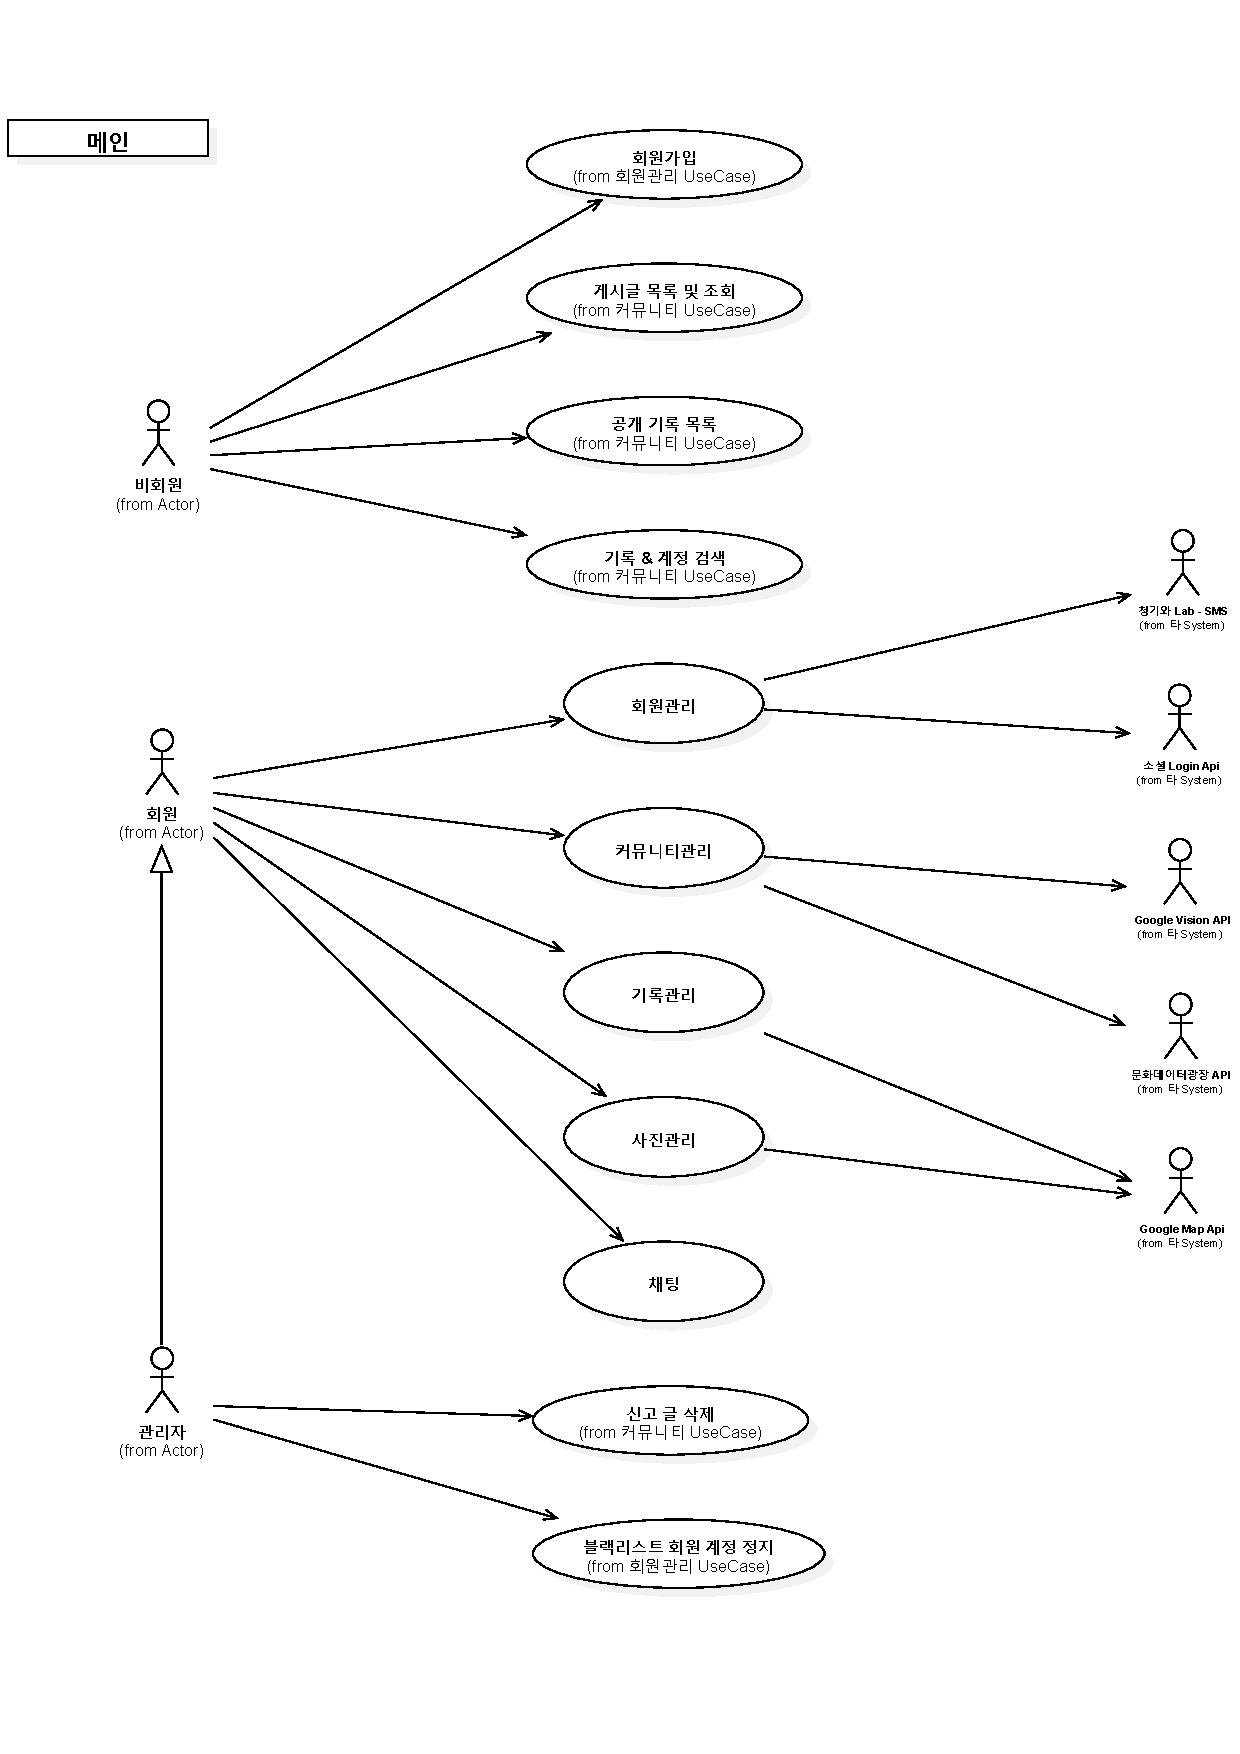
\includegraphics[width=16cm]{./Figure/Analysis/MainUseCaseDiagram.pdf}} \\
    \hline
\end{longtable}
\newpage

\begin{longtable}
    {
        |>{\centering\hspace{0pt}}m{0.300\linewidth}
        >{\raggedleft\hspace{0pt}}m{0.300\linewidth}
        >{\hspace{0pt}}m{0.200\linewidth}|
    } 
    \hline
    \multicolumn{3}{|c|}{\cellcolor{aliceblue}{}} \\
    \multicolumn{3}{|c|}{\cellcolor{aliceblue}{\Large\textbf{Use Case Diagram}}} \\
    \multicolumn{3}{|c|}{\cellcolor{aliceblue}{}} \\
    \hline
    \rowcolor{aliceblue} 
    {\normalsize{시스템 명: Travel Diary}}
    & {\normalsize{작성일: 2020년 12월 21일}}
    & \multicolumn{1}{r|}{\normalsize{작성자: 왕밤빵}} \\ \hline
    \multicolumn{3}{|c|}{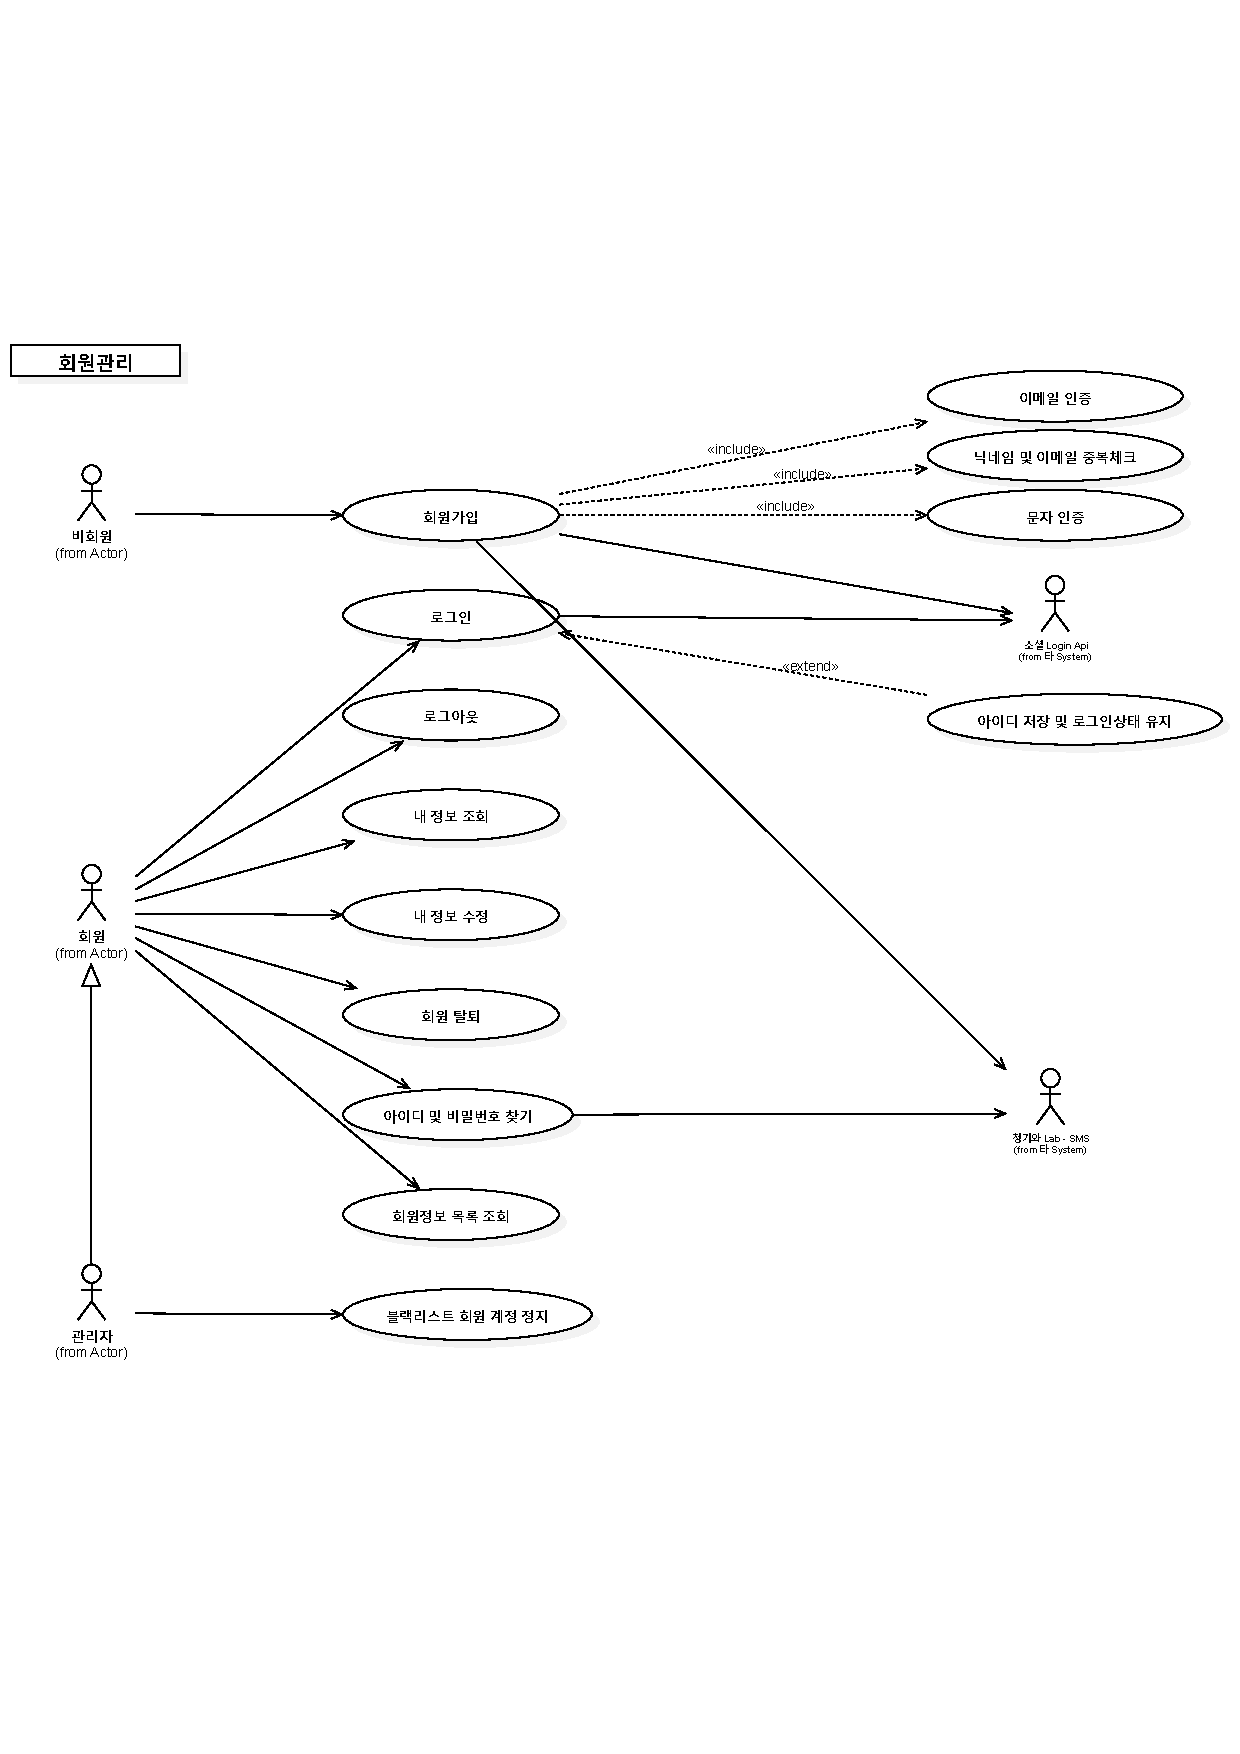
\includegraphics[width=16cm]{./Figure/Analysis/User.pdf}} \\
    \hline
\end{longtable}
\newpage

\begin{longtable}
    {
        |>{\centering\hspace{0pt}}m{0.300\linewidth}
        >{\raggedleft\hspace{0pt}}m{0.300\linewidth}
        >{\hspace{0pt}}m{0.200\linewidth}|
    } 
    \hline
    \multicolumn{3}{|c|}{\cellcolor{aliceblue}{}} \\
    \multicolumn{3}{|c|}{\cellcolor{aliceblue}{\Large\textbf{Use Case Diagram}}} \\
    \multicolumn{3}{|c|}{\cellcolor{aliceblue}{}} \\
    \hline
    \rowcolor{aliceblue} 
    {\normalsize{시스템 명: Travel Diary}}
    & {\normalsize{작성일: 2020년 12월 21일}}
    & \multicolumn{1}{r|}{\normalsize{작성자: 왕밤빵}} \\ \hline
    \multicolumn{3}{|c|}{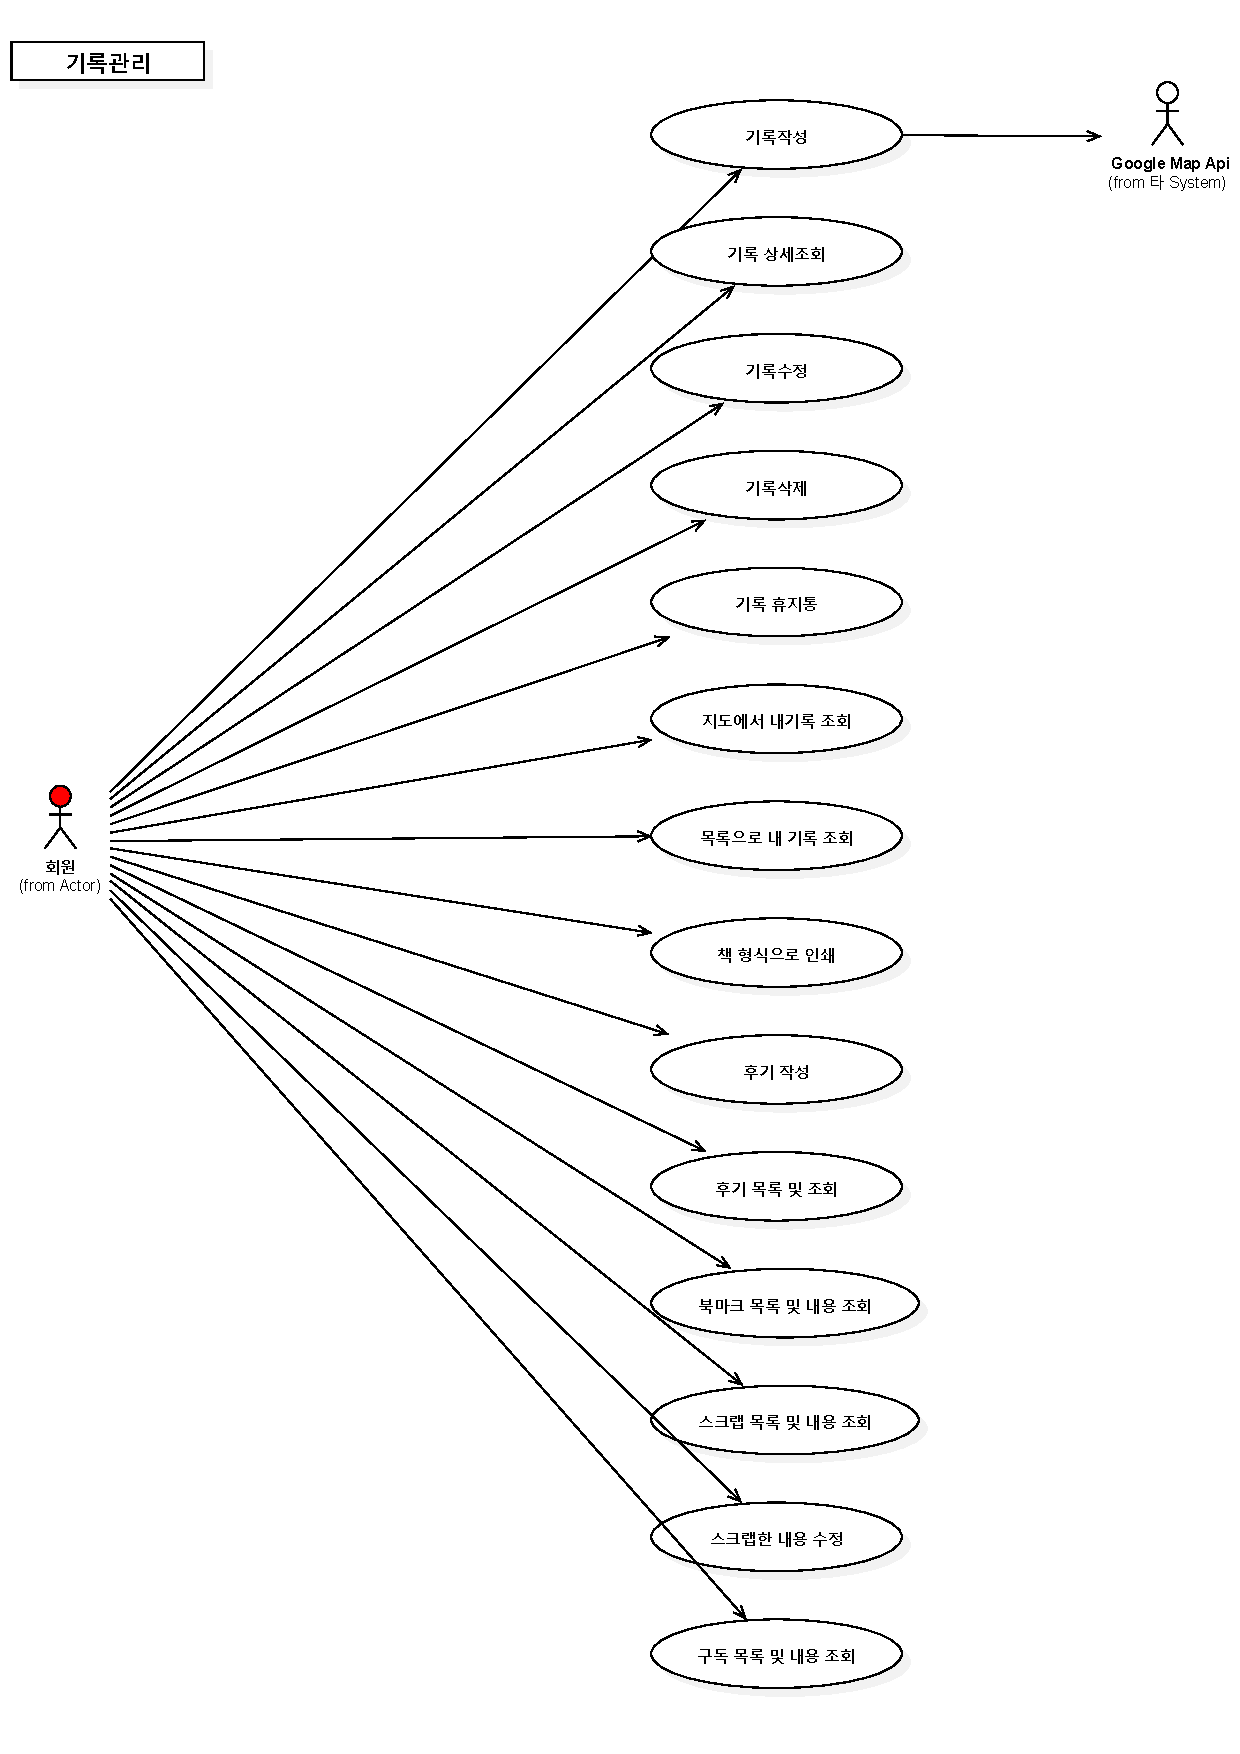
\includegraphics[width=16cm]{./Figure/Analysis/Diary.pdf}} \\
    \hline
\end{longtable}
\newpage

\begin{longtable}
    {
        |>{\centering\hspace{0pt}}m{0.300\linewidth}
        >{\raggedleft\hspace{0pt}}m{0.300\linewidth}
        >{\hspace{0pt}}m{0.200\linewidth}|
    } 
    \hline
    \multicolumn{3}{|c|}{\cellcolor{aliceblue}{}} \\
    \multicolumn{3}{|c|}{\cellcolor{aliceblue}{\Large\textbf{Use Case Diagram}}} \\
    \multicolumn{3}{|c|}{\cellcolor{aliceblue}{}} \\
    \hline
    \rowcolor{aliceblue} 
    {\normalsize{시스템 명: Travel Diary}}
    & {\normalsize{작성일: 2020년 12월 21일}}
    & \multicolumn{1}{r|}{\normalsize{작성자: 왕밤빵}} \\ \hline
    \multicolumn{3}{|c|}{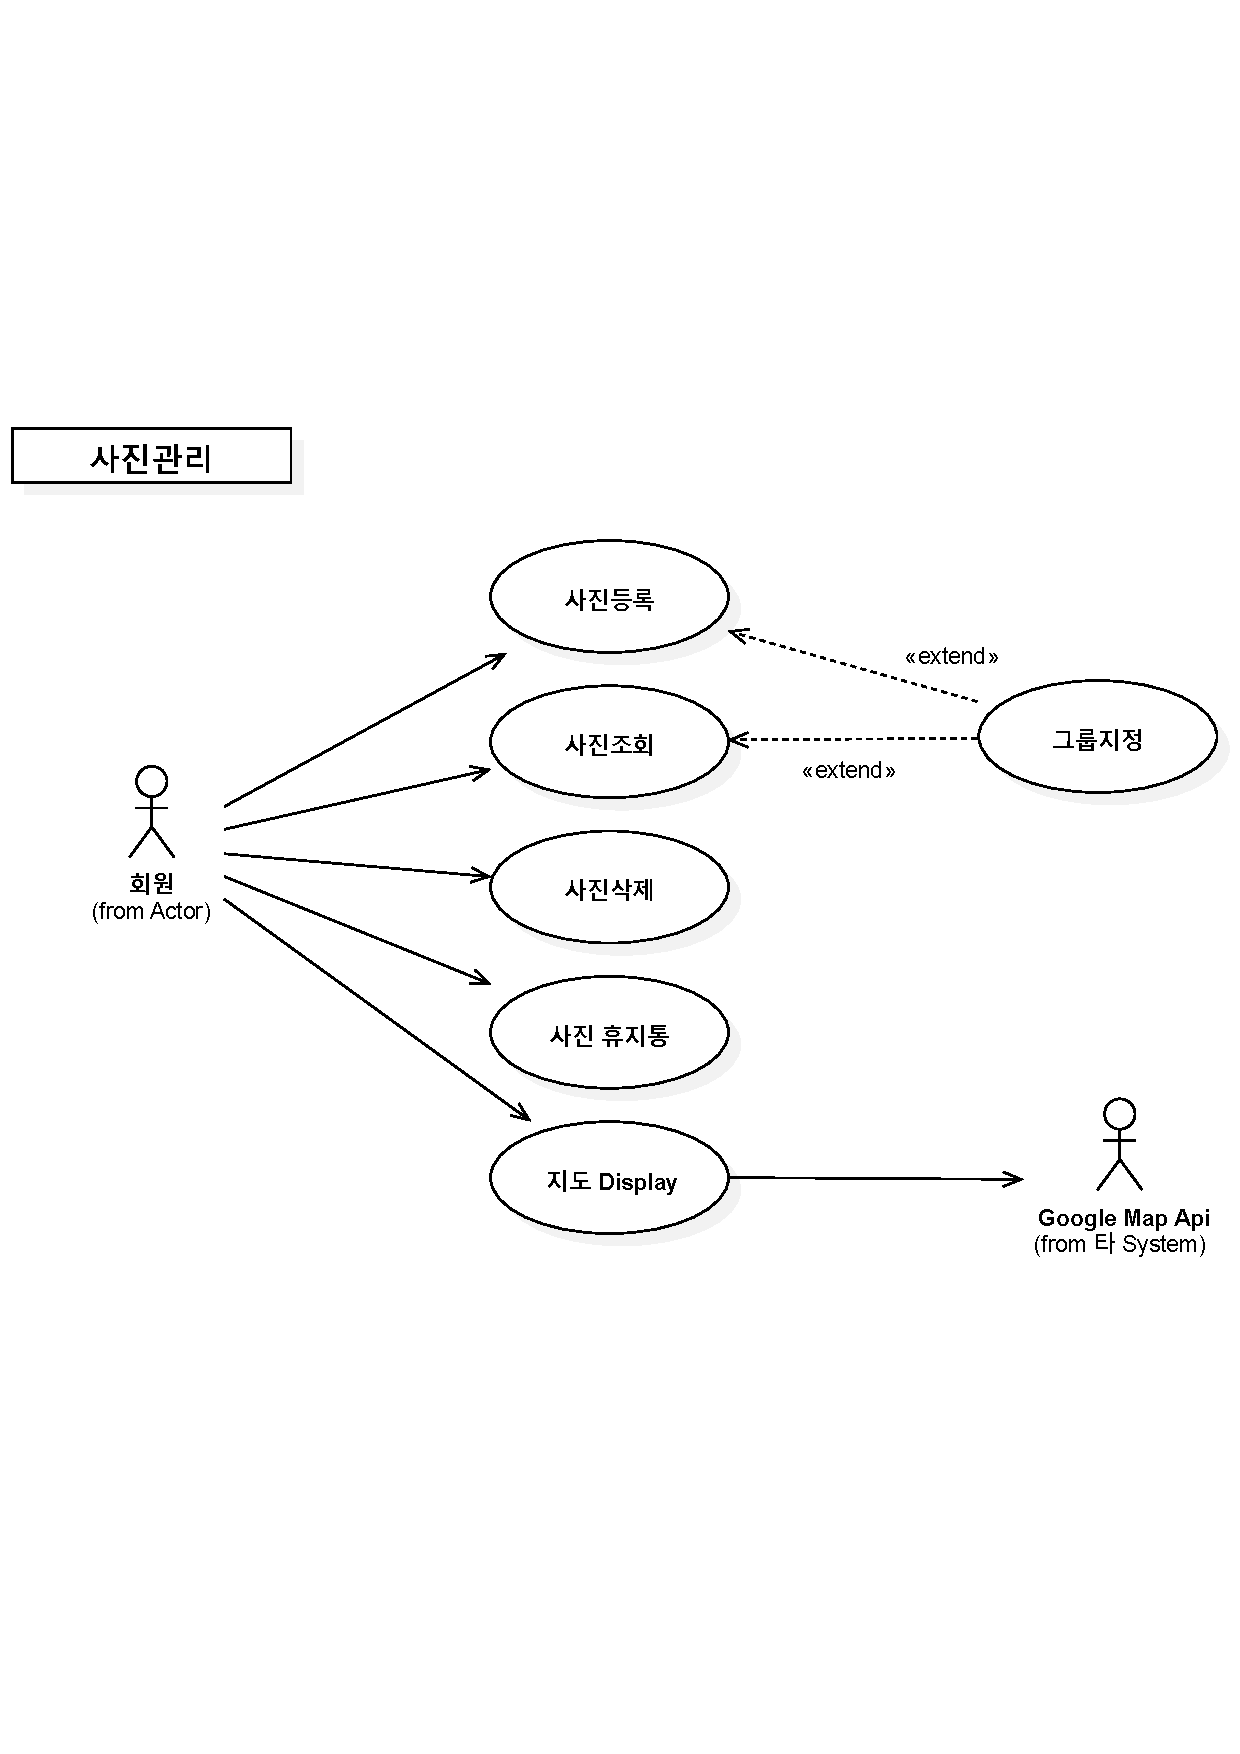
\includegraphics[width=16cm]{./Figure/Analysis/Photo.pdf}} \\
    \hline
\end{longtable}
\newpage

\begin{longtable}
    {
        |>{\centering\hspace{0pt}}m{0.300\linewidth}
        >{\raggedleft\hspace{0pt}}m{0.300\linewidth}
        >{\hspace{0pt}}m{0.200\linewidth}|
    } 
    \hline
    \multicolumn{3}{|c|}{\cellcolor{aliceblue}{}} \\
    \multicolumn{3}{|c|}{\cellcolor{aliceblue}{\Large\textbf{Use Case Diagram}}} \\
    \multicolumn{3}{|c|}{\cellcolor{aliceblue}{}} \\
    \hline
    \rowcolor{aliceblue} 
    {\normalsize{시스템 명: Travel Diary}}
    & {\normalsize{작성일: 2020년 12월 21일}}
    & \multicolumn{1}{r|}{\normalsize{작성자: 왕밤빵}} \\ \hline
    \multicolumn{3}{|c|}{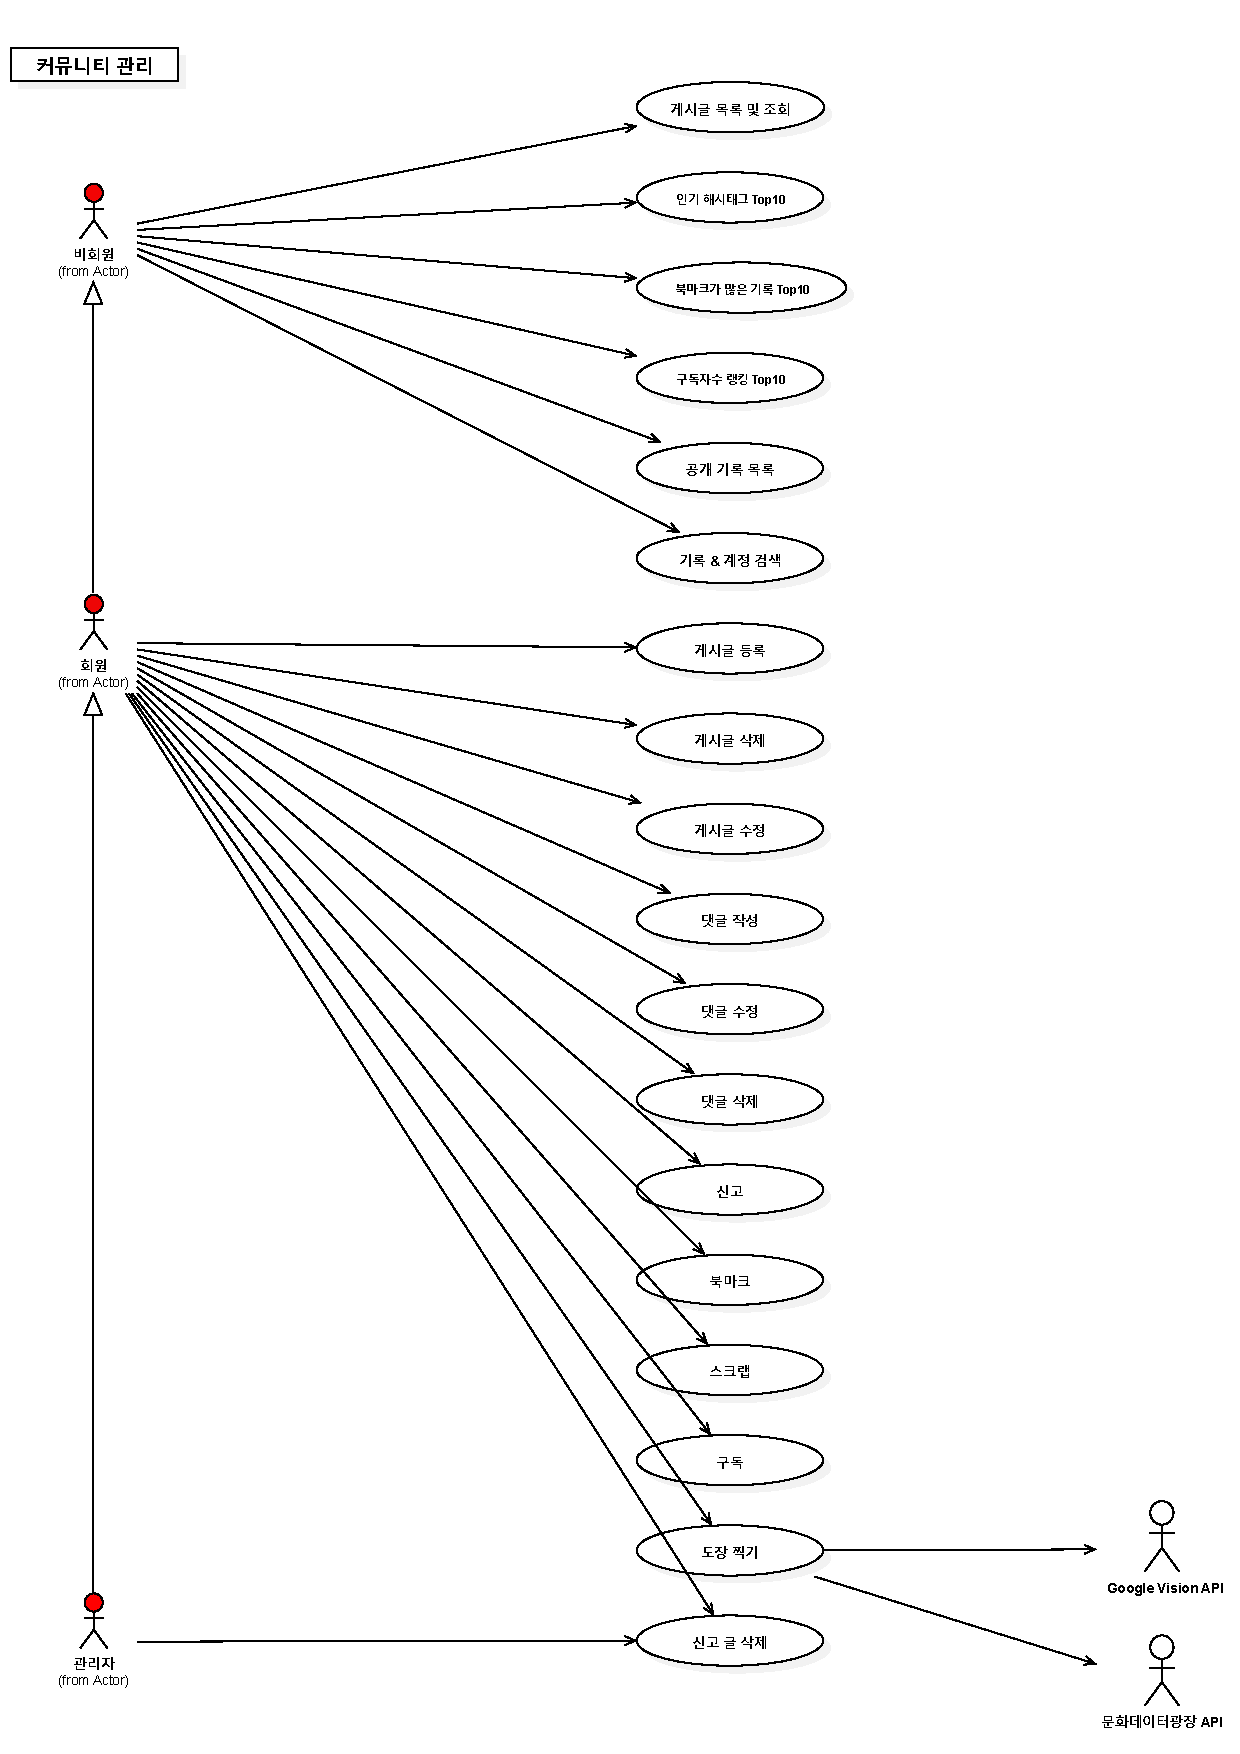
\includegraphics[width=16cm]{./Figure/Analysis/Community.pdf}} \\
    \hline
\end{longtable}
\newpage

\begin{longtable}
    {
        |>{\centering\hspace{0pt}}m{0.300\linewidth}
        >{\raggedleft\hspace{0pt}}m{0.300\linewidth}
        >{\hspace{0pt}}m{0.200\linewidth}|
    } 
    \hline
    \multicolumn{3}{|c|}{\cellcolor{aliceblue}{}} \\
    \multicolumn{3}{|c|}{\cellcolor{aliceblue}{\Large\textbf{Use Case Diagram}}} \\
    \multicolumn{3}{|c|}{\cellcolor{aliceblue}{}} \\
    \hline
    \rowcolor{aliceblue} 
    {\normalsize{시스템 명: Travel Diary}}
    & {\normalsize{작성일: 2020년 12월 21일}}
    & \multicolumn{1}{r|}{\normalsize{작성자: 왕밤빵}} \\ \hline
    \multicolumn{3}{|c|}{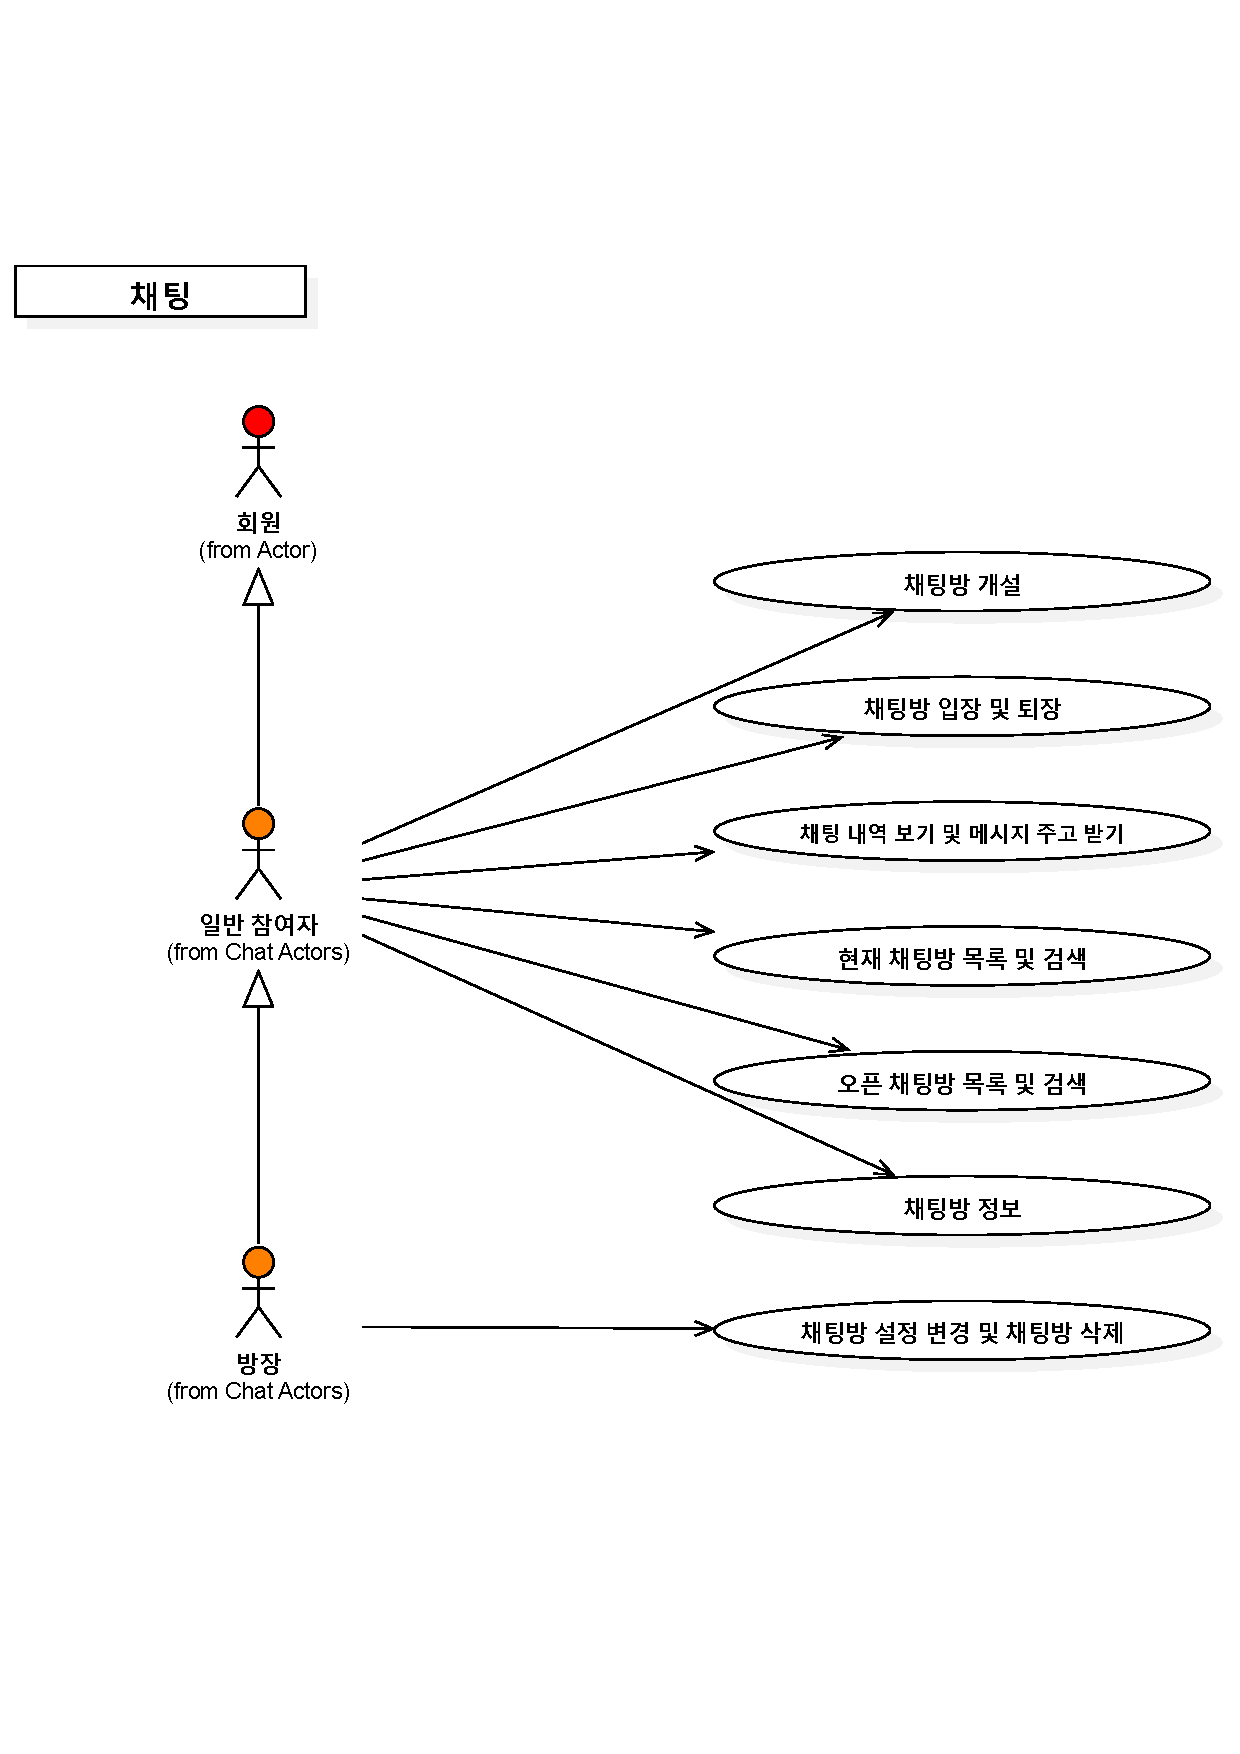
\includegraphics[width=16cm]{./Figure/Analysis/Chat.pdf}} \\
    \hline
\end{longtable}
\newpage


\normalsize
\hiddensection{업무 분석: Application Modeling}
\SectionTitle{\thesection}{업무 분석: Application Modeling}
\begin{enumerate}
    \item In these rules:
    \begin{enumerate}
        \item ...
        \begin{enumerate}
            \item ...
        \end{enumerate}
    \end{enumerate}    
\end{enumerate}

\hiddensection{화면 분석}
\SectionTitle{\thesection}{화면 분석}

\begin{enumerate}
    \item In these rules:
    \begin{enumerate}
        \item ...
        \begin{enumerate}
            \item ...
        \end{enumerate}
    \end{enumerate}    
\end{enumerate}


\hiddensection{데이터 분석(Logical)}
\SectionTitle{\thesection}{데이터 분석(Logical)}

\begin{enumerate}
    \item In these rules:
    \begin{enumerate}
        \item ...
        \begin{enumerate}
            \item ...
        \end{enumerate}
    \end{enumerate}    
\end{enumerate}

\begin{enumerate}
    \item In these rules:
    \begin{enumerate}
        \item ...
        \begin{enumerate}
            \item ...
        \end{enumerate}
    \end{enumerate}    
\end{enumerate}

